


\documentclass[12pt]{article}
\usepackage{natbib}
\usepackage[flushleft]{threeparttable}
\usepackage{longtable}
\usepackage{bm}


\usepackage{listings}
\usepackage[english]{babel}
\usepackage[utf8]{inputenc}
\usepackage[dvips]{graphicx}
\usepackage{amsmath,amsthm,amssymb,tipa,dsfont,mathtools,mathrsfs,here,titlesec,fancyhdr}
\usepackage{anysize}
\usepackage{subfigure}
\usepackage{color}
\usepackage{enumerate}
\usepackage{booktabs}
\usepackage{rotating}
%\usepackage{parskip} % to avoid // 
\usepackage[hidelinks]{hyperref}
\usepackage{url}
\usepackage{multirow}
\renewcommand{\qedsymbol}{\rule{0.7em}{0.7em}}
\usepackage{comment} % begin{comment} to comment large sections
\usepackage[font=scriptsize]{caption}
\usepackage{rotating} % to rotate tables 
\usepackage{tikz}
\usetikzlibrary{shapes,decorations,arrows,calc,arrows.meta,fit,positioning}
\tikzset{
	-Latex,auto,node distance =1 cm and 1 cm,semithick,
	state/.style ={ellipse, draw, minimum width = 0.7 cm},
	point/.style = {circle, draw, inner sep=0.04cm,fill,node contents={}},
	bidirected/.style={Latex-Latex,dashed},
	el/.style = {inner sep=2pt, align=left, sloped}
}

\definecolor{Grey}{RGB}{150, 150, 150}
\definecolor{PPblue}{RGB}{0,114,198}
\definecolor{VOXblue}{RGB}{0,114,198}
\definecolor{PSOEred}{RGB}{232,0,0}
\definecolor{UPred}{RGB}{232,0,0}
\newcommand{\sym}[1]{\rlap{#1}}

\definecolor{mypink}{rgb}{0.858, 0.188, 0.478}
\definecolor{myorange}{rgb}{1.0, 0.49, 0.0}
\definecolor{mypurple}{rgb}{0.6, 0.4, 0.8}
%\usepackage[colorlinks=true,linkcolor=blue,citecolor=blue,hyperfootnotes=false]{hyperref} 
\hypersetup{
	colorlinks,
	citecolor=blue,
	linkcolor=mypink,
	urlcolor=mypurple}
%Els comandaments següents són per a linkejar (han d'estar al final de tots els usepackage)
%\usepackage[colorlinks]{hyperref}%aquests paquets s'utilitzen per a poder linkejar coses.
%\hypersetup{citecolor=red}
%\hypersetup{linkcolor=red}
%\hypersetup{urlcolor=red}
%\usepackage{cleveref}%aquest també.

\usepackage[T1]{fontenc} % for porper quotation marks 
\PassOptionsToPackage{svgnames}{xcolor}
\usepackage{pgfplots}


\usepackage{tcolorbox}
\usepackage{lipsum}
\tcbuselibrary{skins,breakable}
\usetikzlibrary{shadings,shadows}
\newenvironment{myblock}[1]{%
	\tcolorbox[beamer,%
	noparskip,breakable,
	colback=LightBlue,colframe=DarkBlue,%
	colbacklower=DarkBlue!75!LightBlue,%
	title=#1]}%
{\endtcolorbox}

\usepackage{tikz}
\usetikzlibrary{shapes,decorations,arrows,calc,arrows.meta,fit,positioning}
\tikzset{
	-Latex,auto,node distance =1 cm and 1 cm,semithick,
	state/.style ={ellipse, draw, minimum width = 0.7 cm},
	point/.style = {circle, draw, inner sep=0.04cm,fill,node contents={}},
	bidirected/.style={Latex-Latex,dashed},
	el/.style = {inner sep=2pt, align=left, sloped}
}














\renewcommand{\baselinestretch}{1.2} %separació entre linies
\marginsize{2.3cm}{2.3cm}{1cm}{2cm} %Margens


%ací definim els colors que anem a gastar
\definecolor{secction}{rgb}{0.62,0.31,0.00}
\definecolor{subsection}{rgb}{0.33,0.00,0.33}
\definecolor{mygreen}{RGB}{28,172,0}


%S'utilitza per a insertar programes de forma més professional
%\lstset{language=Matlab,numbers=left,frame=single,title=\lstname}
\lstset{language=Matlab,%
    %basicstyle=\color{red},
    breaklines=true,%
    morekeywords={matlab2tikz},
    keywordstyle=\color{blue},%
    morekeywords=[2]{1}, keywordstyle=[2]{\color{black}},
    identifierstyle=\color{black},%
    %stringstyle=\color{mylilas},
    commentstyle=\color{mygreen},%
    showstringspaces=false,%without this there will be a symbol in the places where there is a space
    numbers=left,%
    numberstyle={\tiny \color{black}},% size of the numbers
    numbersep=9pt, % this defines how far the numbers are from the text
    emph=[1]{for,end,break},emphstyle=[1]\color{blue}, %some words to emphasise
    %emph=[2]{word1,word2}, emphstyle=[2]{style},
}

\usepackage[colorinlistoftodos,textwidth=3cm]{todonotes}
\newcommand{\todoINFO}[1]{\todo[color=blue!25]{INFO: #1}}
\newcommand{\todoIMPORTANT}[1]{\todo[color=red!25]{IMPORTANT: #1}}
\newcommand{\todoREV}[1]{\todo[color=green!25]{REVIEWED: #1}}
%Aquí redefinimos los comandos teorema, nota, etc... para que sea más fácil de escribir. Lo que está entre corchetes "[,]" es para que enumere los teoremas en función de la sección, si se quita, lo enumera sobre el total.
\theoremstyle{plain}
\newtheorem{teo}{Theorem}[section]
\newtheorem{prop}{Proposition}[section]
\newtheorem{exe}{Exercise}
\theoremstyle{definition}
\newtheorem{defi}{Definition}[section]
\newtheorem{nota}{Note}
\DeclarePairedDelimiter\abs{\lvert}{\rvert}%
\DeclarePairedDelimiter\norm{\lVert}{\rVert}%
%abreviatures dels comandaments "begin/end". Es una chorradita por no escribirlo todo, puedes usarlo o no.
\newcommand{\be}{\begin{exe}}
\newcommand{\ee}{\end{exe}}
\newcommand{\bt}{\begin{teo}}
\newcommand{\et}{\end{teo}}
\newcommand{\bd}{\begin{defi}}
\newcommand{\ed}{\end{defi}}
\newcommand{\bn}{\begin{nota}}
\newcommand{\en}{\end{nota}}
\newcommand{\bp}{\begin{proof}}
\newcommand{\ep}{\end{proof}}
\usepackage{accents}
\newcommand{\ubar}[1]{\underaccent{\bar}{#1}}

%abreviatures de símbols. Esto en realidad no lo utilizo nunca, pero si te acostumbras es más cómodo.
\newcommand{\e}{\exists}
\newcommand{\fa}{\forall}
%\newcommand{\iff}{\Leftrightarrow}

%Comandaments utilitzats per a donar un millor estil a les pàgines (la xorradeta de la linia de dalt)
\usepackage{fancyhdr}
\pagestyle{fancy}
\lhead{}
%\rhead{Luis Ignacio Menéndez García}
%\renewcommand{\footrulewidth}{0.3pt}

\renewcommand{\headrulewidth}{0pt}   % no line under the header
\renewcommand{\footrulewidth}{0pt}   % no line above the footer


%here we use a new command for the figures titles
\newcommand*{\figuretitle}[1]{%
	{\centering%   <--------  will only affect the title because of the grouping (by the
		\textbf{#1}%              braces before \centering and behind \medskip). If you remove
		\par\medskip}%            these braces the whole body of a {figure} env will be centered.
}

\DeclareMathOperator*{\E}{\mathbb{E}}
\DeclareMathOperator*{\R}{\mathbb{R}}
\DeclareMathOperator*{\Lag}{\mathscr{L}}
\DeclareMathOperator*{\contr}{\Rightarrow\Leftarrow}
\DeclareMathOperator*{\convprob}{\overset{p}{\to}}
\DeclareMathOperator*{\convas}{\overset{a.s.}{\to}}
\DeclareMathOperator*{\convd}{\overset{d}{\to}}
\DeclareMathOperator*{\impose}{\stackrel{!}{=}}



%change colorlinks=false if you don't wan't any hyperlinks to have color

%cmd+n to open a new wnvironment for equation see macros in options of texstudio



%\usepackage[paperwidth=275.9mm, paperheight=279.4mm]{geometry} 
\usepackage{afterpage}
\usepackage{calligra}
\newcommand{\share}{\mbox{\calligra{S}}}

\title{The Impact of Political Campaigns on Demand for Partisan News}
\author{Luis  Menéndez \thanks{Universitat Autònoma de Barcelona, CSIC and Barcelona School of Economics}} %omit the footnote and thanks if needed
\date{\today}

\begin{document}
	\maketitle
	
	\begin{abstract}
		
	How do individuals acquire political information during election campaigns? This paper examines the demand for political news using a unique dataset that combines audience viewership data with the full text of news stories from Spanish TV channels. I estimate a structural random coefficients demand model to capture heterogeneity in political preferences, incorporating demographic differences.
	A key challenge in measuring demand for political content is the endogeneity of news supply. To address this, I propose a novel identification strategy that exploits exogenous variation in the daily news landscape. By classifying all stories produced in Spain on a given day, I construct a set of potential inputs available to TV channels. Since channels have established political stances and face short-run costs in deviating from them, fluctuations in the political composition of available stories constrain left- and right-leaning outlets asymmetrically.
	Using Large Language Models, I categorize the tone of each story with respect to political parties. My findings show that political campaigns significantly alter news consumption patterns. While there is no clear partisan asymmetry in demand before campaigns, polarization emerges once the campaign begins. Right-leaning viewers increasingly seek positive coverage of their own party and negative coverage of the opposition. These results highlight the role of campaign dynamics in shaping media consumption and contribute to the broader literature on political media bias and voter behavior.
		
		
		
		
	\end{abstract}
	
	\clearpage
	
	
	
	\section{Introduction }
	
	

Media plays a crucial role in disseminating information and can influence voting outcomes. Consequently, policymakers often regulate media markets to ensure informational plurality. One common approach is enforcing proportional airtime rules during political campaigns, a policy implemented in several countries.

However, assessing the effectiveness of these regulations requires understanding how viewers respond to the content they consume. Previous research has demonstrated media’s influence on voting behavior during political campaigns \citep{enikolopov}. This issue is particularly relevant in Spain, where political polarization ranks among the highest in Europe, according to recent surveys \citep{edelman_trust_2023}. Notably, affective polarization has increased significantly during our sampling period, raising the question of whether citizens’ political news consumption patterns reflect similar trends.


In this paper, I use a unique dataset that combines Spanish TV news demand from audimeter data with the "product characteristics" of news channels to estimate preferences for political content through a revealed preferences approach; thereby addressing some of the well-known limitations of survey-based studies \citep{prior}.

My analysis focuses on how TV news demand changes during political campaign periods. Previous research has shown that the rise of soft news has contributed to declining interest in political news \citep{patterson2000doing}. Consistent with \cite{gambaro2021revealed}, my findings suggest that periods in which political content is mixed with other types of programming encourage greater audience engagement with politics.

I then investigate the extent of polarized news consumption. Using different machine learning methods, I desing a pipeline that extracts the daily news videos, converts the audio into text and splits the different stories of the day. This methodology allows me to build comparative statics on tone and duration of the same story treated by different outlets on a given day. Using text analysis techniques, I control for the political stance and duration of news stories \citep{puglisi_review}. Specifically, I make use of Large Language Models (LLMs) by inputting all stories into ChatGPT-4, prompting it to identify the tone various political parties. The tone analysis across outlets aligns with viewers' self-reported preferences in survey data, allowing us to classify outlets as left-, right-, or center-leaning based on the parties they most support.

To isolate content choices from demand- or supply-driven factors \citep{gentzkow2011competition}, I assume that news channels engage in a purely horizontal competition, adjusting their content to attract viewers. I then estimate a discrete choice model \citep{berry1994estimating}, in which individuals select their preferred channel based on the political content offered.


In this framework, the political tone offered by news outlets emerges as an equilibrium outcome, making it endogenous in the demand estimation. To address this endogeneity, I exploit random variation in the inputs available to channels. Specifically, I classify all daily news stories produced in Spain during the sample period using data from a major news provider and treat them as the potential story pool for TV outlets. Since channels have established political stances within the differentiation game and face short-run costs in deviating from them, daily fluctuations in the political composition of available stories constrain left- and right-leaning channels differently.

My findings align with previous research on polarized news consumption in the U.S. \citep{Peterson2017Echo}. In the pre-campaign period, there is no systematic asymmetry in political content demand between right- and left-leaning audiences, even when controlling for voting intentions or channel-specific preferences. However, during political campaigns, I find evidence of affective polarization: right-leaning viewers increasingly seek negative coverage of the opposing left-wing party while favoring more positive coverage of their own. This shift in demand coincides with a homogenization of political stances across outlets. Moreover, my results suggest a partisan divide in the overall preference for political content.

This study contributes to the literature on political preferences in media consumption by leveraging exogenous variation in the news landscape to identify political preferences. Notably, my approach relies on unsupervised classification techniques that streamline political categorization. To the best of my knowledge, this is the first paper to examine preferences for political content during campaign periods while explicitly addressing the endogeneity in content supply.



	
	The rest of the paper is organized as follows. In section \ref{section:context}, I briefly summarize the Spanish political and TV landscape. Section \ref{section:data} introduces our data and describes the text analysis techniques we employ, along with some descriptive statistics on both the content and audience sides. In section \ref{section:market}, I describe our market setup and consider the estimation of soft vs. hard news. Section \ref{section:politics} discusses the endogeneity problem and the relevance of our instrument. Results from the demand estimation are shown in section \ref{section:results} Finally, section \ref{sec:supply} shows the current work in progress where I incorporate a supply side estimation.
	
	
	
	
	
	\section{Context} 
	
	\label{section:context}
	
	
	\subsection{Spanish TV market}
	
	Television is still the primary source of information in most European countries \citep{europarl2024}. Figure \ref{fig:motivation} shows the main media used to acquire political information for different European countries, as reported by the 2023 Eurobarometer, broken down by age groups. Television is the preferred medium for almost all age cohorts, a pattern that is even stronger in countries such as France and Italy.
	
	
	
	
	\begin{figure}[h!]
		\centering
		\begin{minipage}[b]{0.45\textwidth}
			\centering
			\textbf{ Spain}
			\includegraphics[width=\textwidth]{figures/media_es}
		\end{minipage}
		\hfill
		\begin{minipage}[b]{0.45\textwidth}
			\centering
			\textbf{ France}
			\includegraphics[width=\textwidth]{figures/media_fr}
		\end{minipage}
		\vfill
		\begin{minipage}[b]{0.45\textwidth}
			\centering
			\textbf{ Belgium}
			\includegraphics[width=\textwidth]{figures/media_be}
		\end{minipage}
		\hfill
		\begin{minipage}[b]{0.45\textwidth}
			\centering
			\textbf{ Italy}
			\includegraphics[width=\textwidth]{figures/media_it}
		\end{minipage}
		\caption{Histogram on the preferred media used for political information in Spain.  
			Source: Eurobarometer, 2022. }
		\label{fig:motivation}
	\end{figure}
	
	
	
	
	The Spanish TV market is a competitive mix of public and private broadcasters, with Televisión Española (TVE) positioned as the state-owned provider of a variety of news, cultural programs, and entertainment. The two primary private conglomerates, Atresmedia and Mediaset, dominate most of the market. Atresmedia operates Antena 3 and LaSexta, while Mediaset controls Telecinco. The mean audience for the channels considered in this study is 2.6 million viewers per day—half a million more than the largest U.S. broadcaster alone: Fox News.
	
	We focus only on the night edition of TV news programs for several reasons. First, it is the so-called "golden time" of the day, attracting the maximum number of viewers on TV. Second, even though channels offer other political programs, the homogeneity of TV news allows us to make very clean comparisons. These programs are broadcast every day at almost the same time and all share a very similar structure, with a presenter introducing the main stories of the day. The well-known informational motives of these shows ensure that people seek to get informed but do so through the outlet that treats news in their preferred way, either due to some perceived outlet quality or differences in the way content is presented.
	
	Altogether, the night editions of these TV news programs capture around $50\%$ of the market share, equating to 8 million viewers, which represents $23\%$ of the potential voting population. For comparison, the average number of viewers for the most popular TV news program in the U.S., Fox News, is around 1.7 million.
	
	
	
	
	
	
	
	\subsection{Political orientation of the audience }
	
	
	Figure \ref{opinion} shows the correlation between political orientation and preferred channel for acquiring political information, based on survey data from the Centro de Investigaciones Sociológicas (CIS). The figure confirms the brief description outlined above. Right-wing individuals (PP-VOX) tend to watch Antena 3 more, whereas left-leaning individuals are divided between LaSexta and the public channel TVE. We can also observe that the correlation with Telecinco initially appears counterintuitive: it attracts viewers from both extremes of the political spectrum, supporting the hypothesis that third factors, such as entertainment, may influence their choice.
	
	\begin{figure}[h!]
		\centering
		\includegraphics[width=160mm]{figures/corr_party_channel3}
		\caption{Source: Built using data from CIS's Encuesta Pre-electoral 2023. The survey ask respondents if they watch TV for political content and what is their preferred channel. Bars represent a correlation coefficient between the declared preferred political party (pooling left and right parties) and the most watched channel. }
		\label{opinion}
	\end{figure}
	
	
	
	Of course, audiences might be politically different because they sort themselves into the channels they like, because they are persuaded by them or, most likely, a combination of both. It goes beyond the scope of this paper to study these effects. 
	
	
	
	
	
	\section{Data and Descriptive Statistics}
	
	\label{section:data}
	
	We have access to a unique dataset that captures both the demand and supply sides of TV news in the Spanish market. For the demand side, I use minute-by-minute viewership data for the four main channels that offer daily TV news programs: TVE, Antena 3, LaSexta, and Telecinco. On the content side, I have daily transcripts that I match to the minute level to see what content people were exposed to. Our data spans from November 2022 to the present, on a daily frequency.
	
	
	
	\subsection*{Audience data }
	
	
	We have high-frequency audience data provided by Kantar Media. For our sample period, I  observe the shares of viewers for each channel on a given day and minute. Although I don't have individual data on choices, I do have geographical disaggregation for the 16 Autonomous regions in Spain, which I will match to survey demographics.\footnote{The Canary Islands and La Rioja are excluded due to different time zones and zero market shares; respectively.}
	
	Furthermore, I match this dataset with one from another media provider, Barlovento. The advantage of this data is that it contains manually annotated sections on a minute-by-minute basis, allowing us to split the unstructured text into different segments of the day. 
	
	The data is pre-processed by first removing the first 5 minutes of the day where audience shifts are likely driven by inertia and not that much to content characteristics. We also homogenize all the outlets to have the same duration and exclude instances in which regions exhibit 0 market shares. 
	
	
	
	\subsection*{TV Content}
	
	I record daily TV news and use Google Cloud infrastructure to store and process the data with \textit{speech-to-text}. Although visuals play a key role in information transmission, I focus only on text transcripts. A more detailed explanation of the entire downloading pipeline can be seen in Appendix Figure \ref{fig:pipeline}.
	
	
	\subsection*{Agencia EFE}
	
	I obtain all news stories provided in Spanish by one of the largest news agencies in the world, Agencia EFE. Due to access limitations, I receive only the title of each story along with a short summary segment. Our sample contains a total of 41K stories.
	
	\subsection*{Survey Data}
	
	To understand polarization behavior, I use survey data gathered from the Centro de Investigaciones Sociológicas (CIS). Specifically, I construct the proportion of people intending to vote for right-wing parties in each Autonomous Community each month.
	
	\subsection*{Weather}
	
	I use meteorological data of daily precipitations per Autonomous Community taken from the Spanish Meteorological Agency (AEMET).
	
	
	\subsection{Political Coverage and Elections}
	
	Political power in Spain has historically been dominated by a two-party system, with either the Socialist Party (PSOE) or the Conservative Party (PP) in power. The emergence of the left-wing party Podemos (UP) following the 15M movement marked a significant shift, as the party began to attract a substantial portion of the electorate.\footnote{Relevant for this period of study is the integration of Podemos into the new political party SUMAR. All classification metrics account for this transition, but throughout the text, I refer to UP as either Podemos or SUMAR after its creation.} Of particular interest is the rise of the far-right party VOX, which made notable gains in the regional elections of 2023, raising the possibility of forming a coalition with the Popular Party (PP) in the regional elections held on May 28, 2023. In response, President Pedro Sánchez decided to bring forward the general elections to June 23, 2023. I refer readers to the \href{https://luisignaciomenendez.github.io/media_monitor/index.html}{Spanish Media Monitor} webpage to explore various metrics of coverage across political parties and actors.
	
	Figure \ref{fig:coverage} shows the average proportion of political mentions in our time period.\footnote{Political mentions are based on dictionaries that include terms for the main political actors and parties.}
	
	\begin{figure}[h!]
		
		\centering
		\includegraphics[width=150mm]{figures/political_words2}
		\caption{Average daily proportion of political terms relative to overall words with shaded standard deviations. Vertical, dashed lines indicate the date of the regional and general elections, respectively. The shaded area represents the "campaign" period considered.}
		\label{fig:coverage}
	\end{figure}
	
	Due to sample restrictions, I divide our time span into two. The \textit{pre-campaign} period starts at the beginning of our data collection in December 2022 and extends to the start of the first publicly announced political campaign on May 13, 2023. The \textit{campaign} period covers both regional and general election campaigns and lasts until the day of the general elections, July 17, 2023.
	
	
	\subsection{ Tone}
	
	
	Do channels align with their viewers' demand in the political content they offer? In this section, I describe the methodology to classify TV content by political leaning. Traditionally, basic text analysis methods, such as measuring mentions or airtime devoted to political actors, have been used to assess plurality and sometimes interpreted as a positive indicator for providing greater publicity. Similarly, sentiment analysis techniques based on semantics cannot reliably discern named entities or context. For this reason, I rely on Large Language Models to classify the stories of the day. The use of LLMs as classifiers has gained popularity in recent years for a variety of context such as classification of political stances \citep{lemens} and has even been found to archive higher precision and accuracy scores for ideological classification when compared to human annotators \citep{tornberg2023}.
	
	Specifically, I use the latest version of ChatGPT-4, feeding it all our political stories and asking it to classify the tone associated with each political party. Notably, I distinguish between positive and negative tones toward the four political parties considered, and I provide a flexible query that allows the classifier to be neutral if the content is ambiguous. More details about the prompt and classification results can be found on Appendix \ref{sec:chat_gpt}
	
	The average tone for each channel-party combination after classification is shown in Figure \ref{fig:chat}. Both Figures \ref{opinion} and \ref{fig:chat} look similar and indicate that viewers self-select into channels that better match their political affiliation—a finding consistent with previous works \citep{gentzkow2011competition} that highlights market equilibrium.
	
	
	
	
	\begin{figure}[h!]
		\centering
		\includegraphics[width=160mm]{figures/chatgpt}
		\caption{Average tone for each channel-party as classified by Chat GPT 4 from the whole sample period. }
		\label{fig:chat}
	\end{figure}
	
	
	
	
	\section{Preferences for Politics}\label{section:politics}
	
	\subsection{Political Tone and Electoral Campaign}
	
	The analysis in the previous sections indicates a general distaste for hard news but does not allow us to comment on tolerance for different political parties. In this section, I explore whether there has been asymmetric distaste for different political parties in response to the campaign period. We begin by detailing how channels have varied their tone toward the parties during this period \citep{independent2023vox}.
	
	We decompose relative tone before and during campaign periods in Figure \ref{fig:tone2}, relative to the number of minutes covered on national politics. The left-leaning channel, LaSexta, significantly reinforced its left position by increasing the positive tone on left-wing parties and decreasing it on both right-wing parties. All other outlets opted for a moderating effect, reducing their mean relative tone.
	
	\begin{figure}[h!]
		\centering
		\includegraphics[width=180mm]{figures/average_tone_pre_post_election}
		\caption{The figure shows the relative tone calculated as the number of minutes pro right minus the number of minutes anti right relative to the total number of minutes devoted to national politics. The vertical dashed line shows results pre and during campaign periods, respectively. }
		\label{fig:tone2}
	\end{figure}
	
	
	
	
	
	\section{Market set up}\label{section:market}
	
	The TV market set up differs from the classical demand estimation problem as there is absence of prices and channels differentiate themselves varying product characteristics. I estimate demand using a mixed logit model \citep{berry1994estimating} \footnote{The model is estimated under the \textit{pyblp} package \citep{conlon2020best}.}.
	
	
	
	An individual $ i $  a given market $ t $ (region-day), chooses an outlet $ j $ based on the following indirect utility : 
	
	
	\begin{equation}\label{eq:utility}
		\begin{aligned}
			& U_{ijt}= \underbrace{\sum_k x_{jt}^k\alpha^k+w_{t}\gamma  +  \xi_{jt}}_{\delta_{jt}}  + \underbrace{  \sum_k x_{jt}^k \Big( \sigma^k \nu_{it}^k  + \pi^ky_{it} \Big)}_{\mu_{ijt}}+\epsilon_{ijt} 
		\end{aligned}
	\end{equation} 
	
	where $ x_{jt}^k $ represents the $ k $th characteristic on channel $ j $ and day $ d(t) $ and $ \sigma^k $ is a shift on characteristic $ k $ mean preferences according to unobserved preferences $ \nu_{i}^k \sim N(0,1)$. For content characteristics we consider the proportion of positive and negative minutes devoted to each party and the relative amount  of minutes spent in political issues to control for a seek of variety in content other than politics.  The exogenous characteristic $w_t$ measures the precipitation on a given day-region. I also introduce as demographics, $ y_{it} $. I use survey data to calculate the proportion of right wing intention to vote in a given region and month. Thus the parameters $\pi^k$ enable us to capture polarization behavior where more right-wing viewers have asymmetric tastes for content on their own and the opposed party tone. 
	
	I decompose the unobserved characteristics into $\xi_{jt}= \xi_j + \xi_{dow} + \Delta \xi_{jt}$, where I include product dummies that account for unobserved quality factors and day of the week dummies to control for the seasonality in our audience data. I also cluster the standard errors at the region level. 
	
	The outside option is modeled in terms of \textit{potential} audience. Formally, the observed share of people consuming a channel  is $ s_{jt}\equiv \frac{q_{jt}}{L_{r(t)}}$where $ q_{jt} $ is the total number of viewers watching channel $ j $ in region-day $ t $ and  $ L_{r(t)} $ is the potential of viewers having access to TV on region $ r(t) $; defined by Kantar media as the population that has access to television in a given region. 
	
	Market shares of channel $j$ on region-day $t$ can be approximated by a sum over the individuals in a given market, $\mathcal{I}_t$ as : 
	
	
	\begin{equation}\label{eq:shares}
		\begin{aligned}
			& s_{jt} = \sum_{i \in \mathcal{I}_t} w_{it} \frac{exp(\delta_{jt} + \mu_{ijt})}{ 1+ \sum_{l\neq j } exp(\delta_{lt} + \mu_{ilt}) } 
		\end{aligned}
	\end{equation} 
	
	
	where $w_{it}$ are survey weights the control for the different relative weight of each region. 
	
	
	
	The nature of the horizontal differentiation game makes product characteristics correlated with unobserved local shocks to viewers' preferences.  I explain in detail our instrumental variables strategy to mitigate this concern in the next section. 
	
	
	
	\subsection{Content endogeneity and News Shocks} \label{section:endogeneity}
	
	
	Under preferences in equation \ref{eq:utility}, content characteristics are an equilibrium outcome of the differentiation game and therefore I expect the  unobserved vertical quality component, $ \xi_{jt} $ to be correlated with them. In this set up, endogeneity arises because local shocks to viewers' preferences are taken into account by the outlets before broadcasting their content. Even though channels cannot adapt content at the region level, Figure \ref{fig:density} shows the political density in the left right spectrum of each channels' audience. Consistent with survey evidence outlined above, channels are aware of their audience composition  and thus internalize political shocks that might affect viewer tastes in a given time period. To address this endogeneity concern, I instrument for each of the $ k $ endogenous product characteristics using supply shocks. 
	
	Suppose that each day contains stories indexed by $ s \in S_d $. A story can be about party $ p(s) \in \{L, R, \emptyset\} $ and have a tone $ \tau(s) \in \{-1, 0, 1\} $ \footnote{Both political but neutral stories and non-political stories are grouped into a tone of 0.}. I define the total number of positive and negative stories available on any given day as the total sum of the tone for $ party \in \mathcal{P}  $ in the News Agency (i.e., Agencia EFE) dataset. Specifically:
	
	
	\begin{equation}\label{eq:first_stage}
		\begin{aligned}
			pos(party)_d^{NEWS}&= \frac{1}{|S_d|} \sum_{s \in S_d}\bigg(\mathds{1}\{\tau(s)=1\} \times \mathds{1}\{p(s)=party\} \bigg)\quad &\forall party \in \{L,R\}\\
			neg(party)_d^{NEWS}&= \frac{1}{|S_d|}\sum_{s \in S_d}\bigg( \mathds{1}\{\tau(s)=-1\} \times \mathds{1}\{p(s)=party\} \bigg) \quad &\forall party \in \{L,R\}\\
			political_d^{NEWS}&=\frac{1}{|S_d|} \sum_{s \in S_d}\bigg(  \mathds{1}\{p(s)\neq\emptyset\} \bigg)
		\end{aligned}
	\end{equation} 
	
	
	I take the equilibrium of the differentiation game as fixed in the short run (i.e., average results from \ref{fig:chat}). This notion of short-run equilibrium is crucial to justify why shocks have product-level variation, even though I take a common set of political stories for all of them. In essence, it is the cost of maintaining the editorial position that makes the day's composition affect outlets differently. This allows  me to place channels on a left-right scale given the \textit{intrinsic ideology} in the differentiation game, as illustrated in Figure \ref{fig:game}. This is crucial as it is the outlet's position \textit{together} with the daily composition of stories $ (pos(party)_d^{NEWS},neg(party)_d^{NEWS}, political_d^{NEWS}) $ that gives variation in news production on both the outlet and market dimensions. 
	
	\begin{figure}
		\centering
		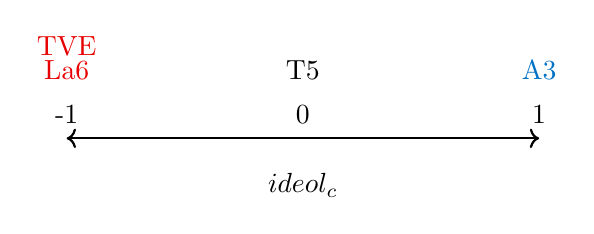
\begin{tikzpicture}
			% Draw the line with arrows
			\draw[<->, thick] (-3,0) -- (3,0);
			
			% Add the numerical labels for -1, 0, and 1
			\node at (-3,0.3) {-1};
			\node at (0,0.3) {0};
			\node at (3,0.3) {1};
			
			% Define positions for the channels
			\node (TVE) at (-3, 0) {};
			\node (La6) at (-3, 0) {};
			\node (T5) at (0, 0) {};
			\node (A3) at (3, 0) {};
			
			% Draw the channel names above the line
			\node[above=0.5cm of TVE] {\textcolor{PSOEred}{La6}};
			\node[above=0.8cm of TVE] {\textcolor{PSOEred}{TVE}};
			\node[above=0.5cm of T5] {T5};
			\node[above=0.5cm of A3] {\textcolor{PPblue}{A3}};
			\node[below=0.2cm of T5] {$ ideol_c $};
			
		\end{tikzpicture}
		\caption{Illustration of the channel's equilibrium position in the political spectrum according to their average reported tone on left and right channels. }
		\label{fig:game}
	\end{figure}
	
	In order to illustrate how the inputs interact with the ideological news production of each outlet, I pool (for simplicity) left channels (La Sexta and TVE), middle (Telecinco) and right (Antena 3) and run regressions of the form: 
	
	
	\begin{equation}\label{eq:pred_pos}
		\begin{aligned}
			pos(p)^{CH}_{jt}=& \sum_{p \in \mathcal{P}} \sum_{j' \in \mathcal{J} }  \left(d(j')_j \times pos(p)^{NEWS} _d      \right) \beta_{j}^{(p,+ )}  + \\
			+ &   \sum_{p \in \mathcal{P}} \sum_{j' \in \mathcal{J} }   \left(d(j')_j \times neg(p)^{NEWS} _d      \right) \beta_{j}^{(p,- )} +\epsilon_{jt}
		\end{aligned}	
	\end{equation} 
	
	
	
	\begin{equation}\label{eq:pred_neg}
		\begin{aligned}
			neg(p)^{CH}_{jt}=& \sum_{p \in \mathcal{P}} \sum_{j'\in \mathcal{J} }    \left(d(j')_j \times pos(p)^{NEWS} _d      \right) \gamma_{j}^{(p,+ )} + \\
			+ &   \sum_{p \in \mathcal{P}} \sum_{j' \in \mathcal{J} }   \left(d(j')_j \times neg(p)^{NEWS} _d      \right) \gamma_{j}^{(p,- )} +\epsilon_{jt}
		\end{aligned}
	\end{equation} 
	
	
	
	\begin{equation}\label{eq:pred_neg}
		\begin{aligned}
			political^{CH}_{jt}=&  \sum_{j'\in \mathcal{J} }\left(d(j')_j \times political^{NEWS} _d      \right)\phi_j +\epsilon_{jt}
		\end{aligned}
	\end{equation} 
	
	
	where $(pos(p)^{CH}_{jt},neg(p)^{CH}_{jt},political^{CH}_{jt} )$  are the analogous to \ref{eq:first_stage} but for each outlet. In this case everything is normalized by the total number of minutes \footnote{Even though the classification of ChatGPT is fed with the splitted stories, I then weight back those stories into the minutes that they span to obtain a measure of how many positive or negative minutes are told by a given outlet in a given day. } 
	
	A positive $ \beta_{ch}^{R,+} $ coefficient indicates that given an extra positive story about the right wing party is available, outlet $ ch $ increases the number of positive stories about that party by $  \beta_{ch}^{R,+}  $, ceteris paribus. 
	
	
	The results of the estimation are shown in table \ref{table:iv_table} on the Appendix. For illustration purposes, I show the predicted production of political stories under different day compositions in figure \ref{fig:prediction2}. I pool parties into left and right groups and  simulate 4 days with the positive/negative combinations for the right and left parties and plot the predicted channel's daily composition. 
	
	Bars represent the difference between the predicted positive and negative  stories for a given party. The top left panel shows that on days highly unfavorable for the left, it is the right channel that presents a more negative scenario for that party. Conversely, days with dominant positive left stories (bottom left graph) only look favorable from the left channels perspective. This illustrates that, even though the shock of news is common to all channels, their intrinsic ideology makes them asymmetrically constrained in their news production and can be used as an instrument. The exclusion restriction implies that audience does not ex-ante react to different composition of the day. For instance, if viewers knew that a scandal happened and they switched to their preferred outlet to watch it, that would violate the identification assumption. Although this cannot be tested directly, I show that using the minute 0 audience (i.e before any content has been shown already), I do not find asymmetric audience gains across outlets based on the composition of the day. Results are shown in appendix table \ref{table:check_exogeneity}.
	
	
	
	
	
	\begin{figure}[ht] 			
		\begin{minipage}[b]{0.5\linewidth}
			\centering
			\includegraphics[width=.9\linewidth]{figures/predicted_bad_left} 
			\vspace{4ex}
		\end{minipage}%%\\
		\begin{minipage}[b]{0.5\linewidth}
			\centering
			\includegraphics[width=.9\linewidth]{figures/predicted_bad_right} 
			\vspace{4ex}
		\end{minipage} 
		\\
		\begin{minipage}[b]{0.5\linewidth}
			\centering
			\includegraphics[width=.9\linewidth]{figures/predicted_good_left} 
			\vspace{4ex}
		\end{minipage}%% 
		\begin{minipage}[b]{0.5\linewidth}
			
			\centering
			\includegraphics[width=.9\linewidth]{figures/predicted_good_right} 
			\vspace{4ex}
		\end{minipage} 
		
		
		\caption{Predicted number of positive minus negative minutes for each outlet and party. The top left (right) plots show days where 4 negative stories for the left(right) party are available and 1 stories of the other type for the rest. The bottom graphs show the analogous scenario with positive stories. 
			The horizontal axis represents the channel classified by its intrinsic ideology into left (La6 and TVE), Middle(Telecinco) and Right (Antena3).  } 
		
		\label{fig:prediction2} 
	\end{figure}
	
	
	For the $ k $ non linear coefficients that represent the variance of the individual heterogeneity I follow \cite{gandhi2019measuring} and target predicted product differentiation instruments of the form $ \left(\hat{x}_{jt}^k- \sum_{l \neq j} \hat{x}_{lt}^k\right)^2 $, where $ \hat{x}_{jt}^k $ is the predicted $ k $th characteristic from the first stage of the instrumental variable regression \ref{eq:first_stage}. To target the demographic parameters, we interact the mean proportion of right votes with those instruments: $ \bar{y}_t\left(\hat{x}_{jt}^k- \sum_{l \neq j} \hat{x}_{lt}^k\right)^2 $.
	
	
	
	
	
	
	\section{Results}
	
	\label{section:results}
	
	
	We present results of the BLP estimation for the pre-campaign and campaign periods in table   \ref{table:results_blp}. We show the preferred specification under outlet and day of the week fixed effects with standard errors clustered at the region level. 
	
	The pre-campaign period estimation shows a significant, positive average taste for negative stories on the right party with significance dispersion ($\sigma_{\text{neg\_right}}$) in the population. Importantly, this dispersion is not explained by ideology heterogeneity ($\pi$ coefficients).
	
	
	
	The campaign period estimates showed at the bottom of the table show a somewhat different set up. There is a significant positive taste for positive stories on the left and negative stories on the right parties. This fact, together with the negative taste on positive right and negative left content would indicate an average preference towards the left leaning parties. The coefficients with the interaction with ideology further indicate a result in line with a polarization behavior: more right wing audiences demand content that is more favorable towards their own party and more negative towards the opposition. The fact that this behavior is exhibited only during the political campaign period and not before links to several results on the political information acquisition.  
	
	The taste for national politics overall is negative with right wing viewers having a higher demand for it. 
	
	
	
	
	\begin{table}[ht]
		\centering
		\begin{threeparttable}
			\begin{tabular}{lccc}
				\hline
				\textbf{Coefficient} & \textbf{Parameter} & \textbf{Estimate} & \textbf{Std. Error} \\
				\hline
				\hline
				\multicolumn{4}{c}{{Pre-campaign}} \\
				\hline
				\hline
				pos\_left & $ \sigma_{\text{pos\_left}} $ & 7.04 & (21.28) \\
				pos\_right & $ \sigma_{\text{pos\_right}} $ & 23.82 & (20.06) \\
				neg\_left & $ \sigma_{\text{neg\_left}} $ & 3.85 & (11.56) \\
				neg\_right & $ \sigma_{\text{neg\_right}} $ & 25.42*** & (5.01) \\
				political & $ \sigma_{\text{political}} $ & 3.47 & (7.58) \\
				\hline
				mean\_right $\times$ pos\_left & $ \pi_{\text{pos\_left}} $ & 21.75 & (16.78) \\
				mean\_right $\times$ pos\_right & $ \pi_{\text{pos\_right}} $ & 35.74 & (43.73) \\
				mean\_right $\times$ neg\_left & $ \pi_{\text{neg\_left}} $ & -48.27 & (33.58) \\
				mean\_right $\times$ neg\_right & $ \pi_{\text{neg\_right}} $ & -63.86 & (48.13) \\
				mean\_right $\times$ political & $ \pi_{\text{political}} $ & -13.89 & (12.77) \\
				\hline
				pos\_left & $ \beta_{\text{pos\_left}} $ & -10.88 & (7.41) \\
				pos\_right & $ \beta_{\text{pos\_right}} $ & -18.19 & (23.08) \\
				neg\_left & $ \beta_{\text{neg\_left}} $ & 14.41 & (12.51) \\
				neg\_right & $ \beta_{\text{neg\_right}} $ & 43.11*** & (16.62) \\
				political & $ \beta_{\text{political}} $ & 4.73 & (5.41) \\
				weather & $ \beta_{\text{weather}} $ & 0.01 & (0.01) \\
				\hline
				\hline
				\multicolumn{4}{c}{{Campaign}} \\
				\hline
				\hline
				pos\_left & $ \sigma_{\text{pos\_left}} $ & 1.26 & (145.13) \\
				pos\_right & $ \sigma_{\text{pos\_right}} $ & 33.40 & (42.70) \\
				neg\_left & $ \sigma_{\text{neg\_left}} $ & 0.38 & (218.79) \\
				neg\_right & $ \sigma_{\text{neg\_right}} $ & 0.54 & (226.19) \\
				political & $ \sigma_{\text{political}} $ & 2.92***& (0.90) \\
				\hline
				mean\_right $\times$ pos\_left & $ \pi_{\text{pos\_left}} $ & -708.11** & (299.27) \\
				mean\_right $\times$ pos\_right & $ \pi_{\text{pos\_right}} $ & 508.87*** & (172.30) \\
				mean\_right $\times$ neg\_left & $ \pi_{\text{neg\_left}} $ & 413.36*** & (147.90) \\
				mean\_right $\times$ neg\_right & $ \pi_{\text{neg\_right}} $ & -455.86** & (178.69) \\
				mean\_right $\times$ political & $ \pi_{\text{political}} $ & 27.60** & (12.62) \\
				\hline
				pos\_left & $ \beta_{\text{pos\_left}} $ & 217.09*** & (76.90) \\
				pos\_right & $ \beta_{\text{pos\_right}} $ & -190.52** & (89.31) \\
				neg\_left & $ \beta_{\text{neg\_left}} $ & -145.58*** & (48.63) \\
				neg\_right & $ \beta_{\text{neg\_right}} $ & 147.49*** & (52.60) \\
				political & $ \beta_{\text{political}} $ & -10.80** & (4.89) \\
				weather & $ \beta_{\text{weather}} $ & 0.04 & (0.03) \\
				\hline
				\hline
			\end{tabular}
			\caption{BLP Estimation Results with Standard Errors \label{table:results_blp_updated}}
			\begin{tablenotes}
				\small
				\item The table shows the results of the BLP estimation of model \ref{eq:utility}. The estimations are divided in the pre-campaign and campaign period. Both day of the week and outlet fixed effects are included. Standard errors are clustered at the region level. total number of observations are $N_{campaign}=2307$ and  $N_{pre\_campaign}=6604$.
			\end{tablenotes}
		\end{threeparttable}
	\end{table}
	
	
	
	
	
	
	The average own-elasticities for each characteristic are shown in table \ref{tab:elasticities_comparison}. Given that increasing the positive relative minutes to a party also implies increasing the overall total minutes on politics, we compute them as:
	
	\begin{equation}\label{eq:elasticities}
		\begin{aligned}
			& \bar{\epsilon}^k= \frac{1}{J_t}\frac{1}{T}\sum_{j}\sum_{t} \left(\frac{\partial s_{jt}}{\partial x_{jt}^k} +  \frac{\partial s_{jt}}{\partial x_{jt}^{political}} \right)\quad \forall k \in \{pos\_right,pos\_left,neg\_right,neg\_left\}
		\end{aligned}
	\end{equation}             
	
	
	
	
	\begin{table}[H]
		\centering
		\begin{tabular}{|l|c|c|}
			\hline
			\textbf{Variable} & \textbf{Pre-Campaign} & \textbf{Campaign} \\
			\hline
			pos\_left & -0.046 & -0.299 \\
			neg\_left & 0.050 & 0.219 \\
			pos\_right & 0.034 & -0.006 \\
			neg\_right & -0.033 & 0.045 \\
			\hline
		\end{tabular}
		\caption{The table shows the estimated elasticities for the political characteristics from equation \ref{eq:elasticities}.}
		\label{tab:elasticities_comparison}
	\end{table}
	
	
	
	

	
	\section{Conclusion}
	
	Understanding the demand of political information is crucial to understand political polarization and media market regulation. However, endogeneity concerns often  impede classical demand estimation techniques due to the lack of valid instruments. In this paper,  I introduce a novel dataset that comprises the Spanish TV market, where I match daily transcripts of the TV news to audimeter data on viewership. I propose a new methodology that makes uses of text analysis and Large Language Models (LLMS ) to analyze the production of political content in TV news. This methodology extracts the political tone and intensity of the daily TV news and  exploits the random availability of political events, together with channel's long-run ideological positions, to measure supply shocks that allow the estimation of  demand preferences.
	
	I show that channels face asymmetric constraints  in their production of political content depending on whether the composition of the day is more or less favorable to their ideological stance. I estimate a structural BLP demand model where I split my sample into both pre-campaign and during political campaign periods. This model allows me to introduce heterogeneity into the demand estimation and decompose political preferences based on the  ideological composition of the audience. My results reveal that while there is no significant asymmetric demand for political content during the pre-campaign period, affective polarization emerges during the political campaign, with right-wing viewers demanding more negative content about the opposing party and more favorable content about their own.
	
	
	
	
	\clearpage
	
	\section{Appendix}
	
	
	
	
	
	
	
	
	
	
	\subsection{Figures}
	
	
	
	\textbf{Pipeline}:
	
	\begin{figure}[H]
		\centering
		\includegraphics[width=150mm]{figures/pipeline3}
		\caption{Pipeline for the text downloading. First videos are downloaded daily from the main TV channels. Google engine is used to convert the audio to text. We then split the stories by minute and user BERTopic to classify and match them. Finally, ChatGPT4 is used to classify political tone.}
		\label{fig:pipeline}
	\end{figure}
	
	
	\begin{figure}[H]
		\centering
		\includegraphics[width=150mm]{figures/average_tone_pre_post_election.png}
		\caption{Average tone for each party and channel pre and during campaign periods}
		\label{fig:party_decomposition}
	\end{figure}
	
	
	\begin{figure}[H]
		\centering
		\includegraphics[width=150mm]{figures/channel_ideology_density_python}
		\caption{Estimated density of channels' audience ideology. The figure shows a kernel density estimate on the ideology score constructed using survey daa and weighted by channels' share of audience for each autonomous region. }
		\label{fig:density}
	\end{figure}
	
	
	
	
	
	
	
	
	\subsection{Chat GPT ideology classification}\label{sec:chat_gpt}
	
	In this section I summarize the usage of ChatGPT as a text classifier for political tone. We detail the prompt and specification details used for the text classification together with final results. 
	
	
	
	
	To reduce both computational and monetary costs, I first filter our split stories using a simple dictionary based approach into those that might contain any relevant political information. Table \ref{table:politics} shows the key terms used to filter the political stories. After the match, I obtain a final number of 15406 political stories that I feed into the chat GPT classifier.
	
	\begin{longtable}{|l|l|l|l|l|}
		\hline
		\textbf{Political} & \textbf{PP} & \textbf{PSOE} & \textbf{SUMAR/UP} & \textbf{VOX} \\
		\hline
		política & pp & psoe & unidas podemos & vox \\
		democracia & partido popular & partido socialista & podemos & abascal \\
		partido político & feijoo & sanchez & ione belarra &de los monteros \\
		gobierno & alberto nunez feijoo & federico buyolo garcia & pablo iglesias & macarena olona \\
		elecciones & ayuso & maria jesus montero & yolanda diaz & ortega smith \\
		votación & cuca gamarra & carmen calvo & irene montero & rocio monasterio \\
		constitución & pablo casado & jose luis abalos & alberto garzon & ignacio garriga \\
		legislación & esperanza aguirre & felix bolanos & iona errejon &jose alcaraz \\
		senado & ana pastor & francina armengol & monica garcia & herminio campillo \\
		congreso & pilar barreiro & sanchez mato & jaume asens & zambrano garcia \\
		dictadura & rafael hernando & margarita robles & noelia vera & luis gestoso \\
		soberanía &alvarez de toledo & marlaska & raul camargo & \\
		estado & javier maroto & jose manuel albares &lopez de uralde & \\
		ciudadanía &  & isabel rodriguez & rosa martinez & \\
		derechos &  &  &  & \\
		libertades &  &  &  & \\
		\hline
		\caption{The table shows the political words included to filter the stories into national politics. We included both general terms that refer to politics as well as party specific terms.}
		\label{table:politics}
	\end{longtable}
	
	
	
	We use OpenAI PI research  using model \textit{gpt-4-0125-preview} to build queries of the form: 
	
	
	\begin{tcolorbox}[colback=blue!5!white, colframe=blue!75!black, title=Prompt]
		Analyze the sentiment of the following news article with respect to the political parties (and their members) in Spain: PP, Podemos/Sumar, PSOE, VOX. Only use numeric values from the set [-1, -0.5, 0, 0.5, 1].
		
		Evaluate the sentiment towards each party with a number between -1 and 1, where -1 indicates an extremely negative perception, 0 indicates neutrality or irrelevance for the party, and 1 indicates an extremely positive perception.
		
		Consider only the values -1, -0.5, 0, 0.5, and 1.
		
		Base your evaluation solely on the explicit content of the news article. If the article does not mention or imply any sentiment towards a party, assign a 0 to that party.
		
		The format must always be a list \texttt{[PP
			, PSOE
			, UP
			, VOX
			]} where \texttt{X} represents the numeric sentiment value.
		
		
	\end{tcolorbox}
	
	
	Due to the stochasticity in LLMs predictions, good practices recommend to run the classification multiple times and avere out the results \citep{tornberg2023}. Financial costs, however, impede us from doing the whole approach multiple times but I show results on stability below on a subset of stories. 
	
	Results of the final classification for the non neutral stories are shown in figure \ref{fig:sent_distribution}. Each bar represents the percentage of stories of that given sentiment associated to each political party. We can see that the classification reserved the extreme values 1 and -1 for few stories and focused on the -0.5 and 0.5 values. 
	
	
	
	\begin{figure}[H]
		\centering
		\includegraphics[width=120mm]{figures/sentiment_distribution}
		\caption{The figure shows the percentage of stories to each political party for a given sentiment. We exclude neutral stories.}
		\label{fig:sent_distribution}
	\end{figure}
	
	
	\begin{table}
		
		\centering
		\begin{tabular}{lrrrr}
			\hline
			Statistic       &       PP &     PSOE &      VOX &       UP \\
			\hline
			Mean            & -0.013759 &  0.106458 & -0.053395 &  0.024250 \\
			Standard Error  &  0.003166 &  0.003582 &  0.001345 &  0.001970 \\
			\hline
			
		\end{tabular}
		
		\begin{tablenotes}
			\centering
			\footnotesize
			\item Note: The table shows the mean and standard error for 100 rounds of Chat GPT classification of political with 40 random political stories.
		\end{tablenotes}
	\end{table}
	
	
	
	
	
	\subsection{Instrument validity}
	
	
	The instrumental variable approach outlined in section \ref{sec:endogeneity} relies on the assumption that the supply shifters are uncorrelated to demand. This assumption would be violated if viewers exhibit some anticipation behavior. For example, individuals might get information about what has happened on a given day and tune into the channel they prefer accordingly. Although this cannot be tested directly, I propose a simple test of this behavior in a reduced form approach. We want to see if the minute 0 audience is correlated to the political composition of the day. By considering the initial audience, I make sure that channel's content has not play a role yet. Specifically, I run channel by channel regressions of the form: 
	
	\begin{equation}\label{eq:check_exogeneity}
		\begin{aligned}
			ln\left( \frac{q_{crd}}{L_{r}-Q_{rd}}  \right) = \beta_0 + \sum_{p \in \{L,R\}}\left(\beta_p pos(p)^{NEWS}_d + \beta_p neg(p)^{NEWS}_d \right)+ \beta_{pol} pol^{NEWS}_d + \gamma_{dow} + \gamma_r + \epsilon_{crd}
		\end{aligned}
	\end{equation} 
	
	
	
	
	\begin{table}
		\centering
		{
\begin{tabular}{l*{4}{c}}
\hline
&\multicolumn{4}{c}{$   ln\left( \frac{q_{crd}}{L_{r}-Q_{rd}}  \right)$}\\
\hline
          &\multicolumn{1}{c}{(1)}&\multicolumn{1}{c}{(2)}&\multicolumn{1}{c}{(3)}&\multicolumn{1}{c}{(4)}\\
          \hline
\hline
pos\_right\_news&  -1.1830\sym{***}&  -1.2970\sym{***}&  -0.9093\sym{***}&  -0.9572\sym{***}\\
          & (0.2379)         & (0.2059)         & (0.2365)         & (0.2832)         \\
pos\_left\_news&   0.2434         &   0.8154\sym{***}&   0.6709\sym{***}&   0.6657\sym{***}\\
          & (0.2172)         & (0.1709)         & (0.2461)         & (0.2339)         \\
neg\_right\_news&  -0.6172\sym{***}&  -0.7594\sym{***}&  -1.0197\sym{***}&  -0.5473\sym{**} \\
          & (0.2177)         & (0.1771)         & (0.2712)         & (0.2548)         \\
neg\_left\_news&   1.5192\sym{***}&   1.7982\sym{***}&   1.0508\sym{***}&   1.0127\sym{***}\\
          & (0.2582)         & (0.2026)         & (0.2770)         & (0.2861)         \\
political\_news&  -0.5071\sym{**} &  -0.5051\sym{***}&   0.0565         &  -0.3992\sym{*}  \\
          & (0.2029)         & (0.1723)         & (0.2213)         & (0.2388)         \\
\_cons     &  -3.3131\sym{***}&  -2.7860\sym{***}&  -3.6418\sym{***}&  -4.1093\sym{***}\\
          & (0.0650)         & (0.0546)         & (0.0671)         & (0.0724)         \\
\hline
\(N\)     &     2231         &     2555         &     2001         &     2381         \\
\hline\hline
\multicolumn{5}{l}{\footnotesize Standard errors in parentheses}\\
\multicolumn{5}{l}{\footnotesize \sym{*} \(p<0.10\), \sym{**} \(p<0.05\), \sym{***} \(p<0.01\)}\\
\end{tabular}
}

		\caption{The table shows the results from the estimation of \ref{eq:check_exogeneity} conditional on minute 0 audience. Each column represents the regression on channels TVE, A3, Telecinco and La Sexta ; respectively. Day of the week and region fixed effects are included. }
		\label{table:check_exogeneity}
	\end{table}
	
	
	Table \ref{table:check_exogeneity} show the estimated coefficients from equation \ref{eq:check_exogeneity} where each column corresponds to a separate outlet regression and I condition on our minute zero audience. Equation \ref{eq:check_exogeneity} is the linear analogue of a logit estimation. The consistent sign of the coefficients across the different covariates indicates that viewers might not strategically choose across the outlets as a function of what the stories of the day were. This, however, doesn't preclude strategic substitution towards the outside option. 
	
	
	
	
	
	\subsection{Alternative methods for segment splitting in unstructured text}
	
	We explain here different unsupervised text splitting methods that were tried to split the segments of the day. To the best of our knowledge, these methods have not been applied before and can be easily extended to any TV news set up. The advantage of these techniques is that they provide an unsupervised way to split unstructured text into stories that is precise up to the second level, thus overcoming the problem of the manually annotated labels which goes at the minute level. There is, however, computational or financial costs in some of them that impeded us to use them for our whole dataset.
	
	\textbf{Image recognition}
	
	Outlets typically segment their sections by means of captions where they introduce headers for the upcoming story. Exploiting our video dataset, I designed an unsupervised image recognition algorithm that tracks the appearance of those new segments and produces a set of times that serve as text splitters. Although precise, the disadvantage of this method is that it remains computationally intensive as videos need to be segmented and then processed into the algorithm. Computational cost can be reduced by focusing on the lower bottom of the screen  only (figure \ref{figure:image_rec}), which is the area where the output is expected to appear.
	
	\begin{figure}[H]	\label{figure:image_rec}
		\centering
		\includegraphics[width=100mm]{figures/image_recog}
		
		\caption{Example of a image with a caption that delimits the beginning of a new section. The highlighted area shows the bottom of the image where image recognition can be applied to find such appearances.}
		
	\end{figure} 
	
	
	
	
	\textbf{Speaker diarization}
	
	
	A less computationally expensive alternative consist on using \textit{speaker diarization} on the wav files. After transforming the mp4 file to audio using \textit{ffmpeg}, I use Google Cloud diarization tool to find the different speakers in an audio file. The most common (or most two common if it is a weekend) speakers overall corresponds to the presenter of the news. After allowing a flexible specification, one can identify break points by cheeking the seconds where the presenter comes back into scene making sure she is speaking long enough so that a new segment is being introduced. Figure \ref{fig:diarization} illustrates this procedure and the comparison with the manually annotated labels for an example day-channel.
	
	
	\begin{figure}[H]
		\centering
		\includegraphics[width=120mm]{figures/speakers_all}
		\includegraphics[width=120mm]{figures/speaker_timeline}
		\caption{The top figure shows the timeline for the presenter audio (red) vs other audios recognized by \textit{speech2text} in a wav file for the 15th January 2023 in La Sexta. Vertical, black, dashed lines represent the predicted splits based on the diarization. The bottom figure combines these splits with the ones that come from the manually annotated figures. Red, dashed bars correspond to the breaks that come from the manually annotated GECA dataset. Green bars represent breaks where both the speaker diarization and the manual annotation coincide on a break. }
		\label{fig:diarization}
	\end{figure}
	
	
	
	
	%\nocite{*}
	\clearpage
	%\addcontentsline{toc}{chapter}{Bibliography}
	%\printbibliography
	
	\addcontentsline{toc}{chapter}{Bibliography}
	\bibliographystyle{apa}
	\bibliography{./bib/media_bias.bib}
	
	
	
	
	
	
	
	
	
	
	
	
\end{document}